%!TEX root = M1P1.tex

\stepcounter{lecture}
\setcounter{lecture}{4}

\pagebreak

\sektion{Differentiation}
\label{sub:differentiation}

\subsektion{Differentiability}\vspace*{5pt}

\begin{definition}
$f$ is \emph{differentiable}  at $a$ iff $\lim_{x\to a} \frac{f(x)-f(a)}{x-a} = f'(a)$, i.e.
\[\forall \epsilon > 0,~\exists \delta > 0\text{ such that } 0<|x-a| < \delta \implies \left|\frac{f(x)-f(a)}{x-a}-f'(a)\right| < \epsilon.\]	
\end{definition}

\begin{center}
\begin{tikzpicture}
\begin{axis}[
 axis line style={red},
 axis lines=middle,
  ymin = -0.2,
  ymax = 1,
  xmin = 4,
  xmax = 10,
     ytick = 0,
   xtick = 0,
  width=12cm,height=6cm]
      \addplot[draw=blue, domain=4:9,smooth]{0.006*x^4 - 0.0987*x^3 + 0.3937*x^2 + 0.6556*x - 3.9};
       \draw (axis cs:7.7,0.53) -- (axis cs:8.2,0.65); %tangent line
       \draw (axis cs:8.2,0.65) -- (axis cs:8.2,-0.04) node at (axis cs: 8.2,-0.1) {$x$};
       \draw (axis cs:7.7,0.53) -- (axis cs:7.7,-0.04)  node at (axis cs:7.7,-0.1) {$a$};
        \draw[<->] (axis cs:8.3,0.53) -- (axis cs:8.3,0.65) node at (axis cs: 8.9,0.6) {\small $f(x) - f(a)$};
         \node[text width=4cm] at (axis cs:7.5,0.8) {\small straight line gradient $= \frac{f(x)-f(a)}{x-a}$};
  \end{axis}
\end{tikzpicture}
\end{center}

\begin{example}
$f(x) = x^2$ is differentiable at all $a \iR$ with $f'(a) = 2a$
\begin{proof}
Fix $a\iR$
\[\frac{f(x) -f(a)}{x-a} = \frac{x^2 -a^2}{x-a} = x+a\]
\[\implies \lim_{x\to a} \frac{f(x) -f(a)}{x-a}\text{ exists and equals } 2a\]	
\end{proof}	

or from first principles:
\[\left|\frac{f(x) -f(a)}{x-a}-2a\right| = |x+a-2a| = |x-a|\]
So fixing $\epsilon >0$, take $\delta = \epsilon$ so that $|x-a| < \delta \implies \left|\frac{f(x) -f(a)}{x-a} - 2a\right| < \epsilon$ \qed
\end{example}

Exercise: $f(x) = x^3$, $f(x) = |x|$\\

\begin{proposition}\lecturemarker{26}{13 March}
If $f$ is differentiable at $a\iR$ then $f is$ continuous at $a$	
\end{proposition}

\begin{proof}[Proof] If $f$ is differentiable at $a$ then
	\[\begin{aligned}\forall \epsilon >0~ \exists \delta  > 0 \text{ such that } 0 < |x-a| < \delta &\implies \left|\frac{f(x) - f(a)}{x-a} - f'(a)\right| < \epsilon \\ 
	&\implies |f(x) - f(a)| < |x-a|(|f'(a)| + \epsilon).	
\end{aligned}
\] 
	Fix $\epsilon > 0$, set $\delta = \epsilon$. Then \[0 < |x-a| < \delta \implies  |f(x) - f(a)| < \epsilon(|f'(a)| + \epsilon) = k\epsilon\] (also true for $x = a \implies |f(x) - f(a)| = 0$.)
\end{proof}

\begin{proof}[Highbrow Proof]
Note that $f(x) = f(a) + (x-a)\frac{f(x) -f(a)}{x-a}$, $x \neq a$. Taking  $\lim_{x\to a}$  \[\lim_{x\to a}f(x) = f(a) + 0.f'(a) \implies f \text{ cts at } a\qedhere\]\end{proof}

The converse is \emph{not} true.\vspace*{10pt}

\begin{example}
$f(x) = |x|$ is continuous at $x = 0$ but not diff'ble at $x = 0$ since 

\[\frac{f(x) -f(0)}{x-0} = \frac{|x|}{x} = \begin{cases}
 1 & \text{ if } x > 0\\
 -1 & \text{ if } x < 0	
 \end{cases}
\]
So $\lim_{x\to o} \frac{f(x) -f(0)}{x-0}$ does not exist (Ex)

\begin{center}
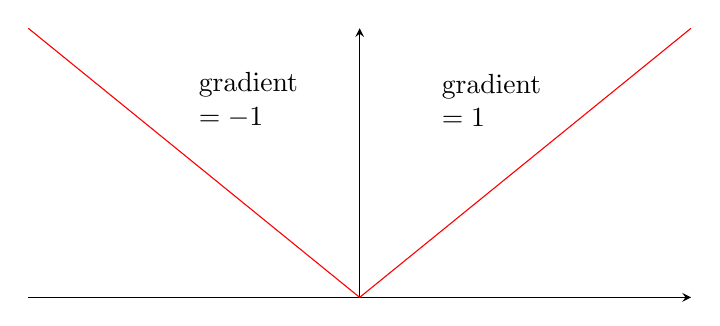
\begin{tikzpicture}
\begin{axis}[
axis lines=middle,
xtick = {0},
xticklabels = {$0$},
ytick = 0,
  width=10cm,height=5cm]
   \addplot[color = red, domain=-0:0.003,smooth]{x};
   \addplot[color = red, domain=-0.003:0,smooth]{-x};
   \node[text width = 1cm] at (axis cs: 0.0011,0.0022) {gradient  $= 1$};
   \node[text width = 1cm] at (axis cs: -0.0011,0.0022) {gradient $= -1$};
 \end{axis}
\end{tikzpicture}
\end{center}




So left and right derivates do exist, they're just not equal. 
\end{example}\vspace*{5pt}

\begin{definition}
Left derivative of $f$ at $a$ is $\lim_{x \to a^-}\frac{f(x) -f(a)}{x-a}$ iff it exists. Right derivative is $\lim_{x \to a^+}\frac{f(x) -f(a)}{x-a}$. 

$\lim_{x \to a^-}g(x)$ exists and equals $\lim_{x \to a^+}g(x) \iff \lim_{x\to a}g(x)$ exists.
\end{definition}

So $f$ is differentiable at $a$ iff the left and right derivatives of $f$ exist at $a$ and are equal. 

Anything else you might guess is also false: e.g. ``if $f$ is differentiable everywhere then is $f'$ continuous?'' No!\vspace*{10pt}

\begin{theorem}[Product Rule] $f,g : \RR \to \RR$ differentiable at $a \in \RR$. Then $fg$ is differentiable at $a$ with $(fg)'(a) = f'(a)g(a) + f(a)g'(a)$
\end{theorem}
\begin{proof}
\[\begin{aligned}
	\frac{f(x)g(x) - f(a)g(a)}{x-a} &= \frac{(f(x)-f(a))g(x) + (g(x) - g(a))f(a)}{x-a} \\ 
	&= g(x) \frac{f(x)-f(a)}{x-a} + f(a)\frac{g(x)-g(a)}{x-a}
\end{aligned}
\]
Taking $\lim_{x\to a} \implies (fg)'(a) = g(a)f'(a) + f(a)g'(a)$ by cty of $g$ and algebra of limits.
\end{proof}
\pagebreak

\begin{corollary}
$f(x) = x^k$ has $f'(x) = kx^{k-1}$	
\end{corollary}
\begin{proof}
Induction!	
\end{proof}

Then $g(x) := 1/f(x)$ is defined in a neighbourhood of $a$, and it is differentiable with $g'(a) = \dfrac{f'(a)}{f^2(a)}$

\begin{proof}
See old question sheet.

 $f$ is continuous at $a \implies \exists \delta > 0$ s.t. $\forall x \in (a-\delta,a+\delta),~|f(x)| > \frac{|f(a)|}{2}$. So $g$ is defined on $(a-\delta,a+\delta)$. 
 
 Working on this and $(a-\delta,a+\delta)\ni x$ we calculate
 
 \[\begin{aligned}\frac{g(x) -g(a)}{x-a} &= \dfrac{1/f(x) -1/f(a)}{x-a}\\
 &= \frac{f(a) - f(x)}{(x-a)f(a)f(x)}\\
 &\to -f'(a)\cdot\frac{1}{f(a)f(a)} \text{ as } x \to a
\end{aligned}\]
\end{proof}


\begin{example}
$E(x) = \sum_{n=0}^\infty \frac{x^n}{n!},~x\iR$	

If we could differentiate term by term we would conclude that

\[E'(x) = \sum_{n=1}^\infty \frac{nx^{n-1}}{n!} = \sum_{k=0}^\infty \frac{x^k}{k!} \quad(k=n-1)\]
So Mestel \emph{guesses} that $E' = E$

\textbf{Claim:} $E'(0) = 1$
\begin{proof}
\[\begin{aligned}\frac{E(x) -E(0)}{x-0} &= \frac{\sum \frac{x^n}{n!}}{x}\\
&= \sum_{n=1}^\infty \frac{x^{n-1}}{n!}\\
&= 1 + \sum_{k=1}^\infty \frac{x^k}{(k+1)!} \quad(k = n+1)
\end{aligned}
\]

Now by the comparison test \[\sum_{k=1}^\infty \frac{x^k}{(k+1)!} \leq \sum_{k=1}^\infty |x^k| = \dfrac{|x|}{1-|x|} \to 0\]

So $\lim_{x\to 0} \dfrac{E(x) - E(0)}{x-0}$ exists and equals $1$. 
\end{proof}

So now we have
\begin{proposition}
$E$ is differentiable everywhere with $E' = E$	
\end{proposition}
\begin{proof}

\[\begin{aligned}
\frac{E(x) - E(a)}{x-a} &= E(a)\cdot \frac{E(x-a)-E(a)}{x-a}\\
 &\to E(a)E'(0) \\
&= E(a)	
\end{aligned}
\]	
\end{proof}
\end{example}\vspace*{15pt}


\subsektion{Rolle's Theorem}\vspace*{5pt}


\begin{theorem}[Rolle's Theorem]\lecturemarker{27}{16 March}
	$f:[a,b] \to \RR$ cts on $[a,b]$, differentiable on $(a,b)$ such that $f(a) = f(b)$. Then $\exists c \in (a,b)$ such that $f'(c) = 0$.
\end{theorem}



\begin{center}
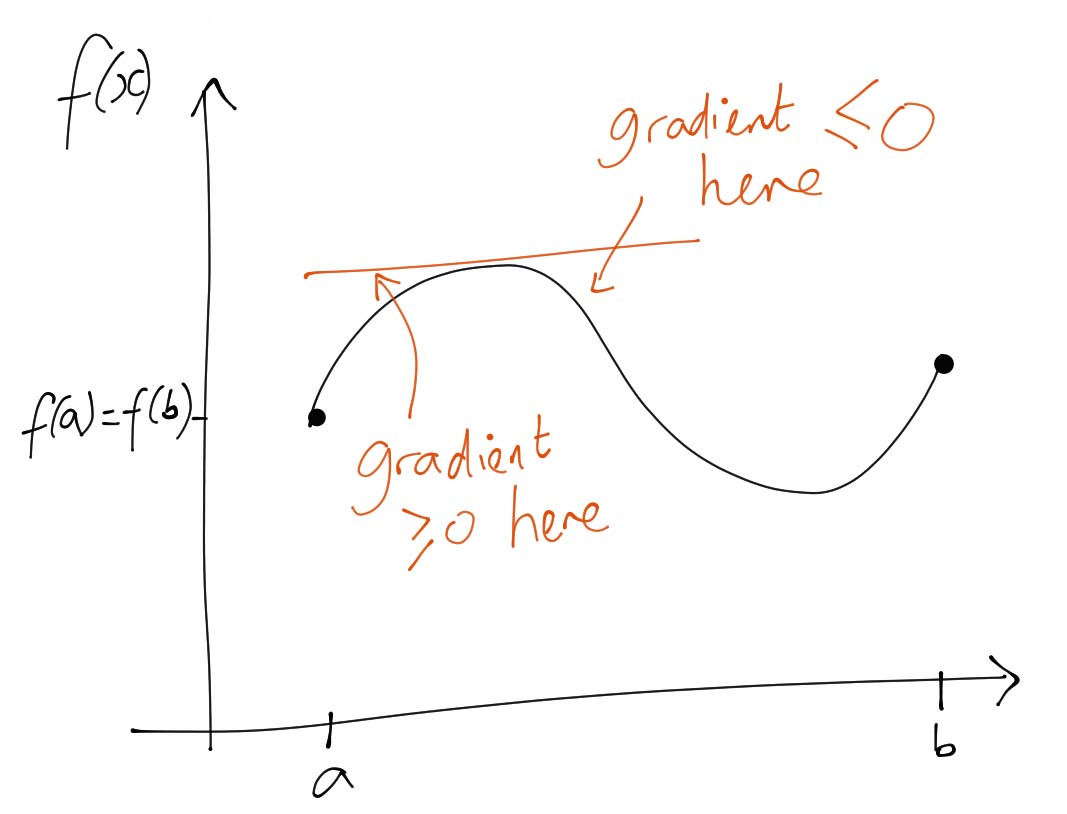
\includegraphics[width = 8cm]{rolle.jpg}
\end{center}


\begin{proof}~
\begin{enumerate}
\item[Case 1.] $f$ is constant on $[a,b]$. Then set $c = \frac{a+b}{2},$ so $f'(c) = \lim_{x\to c}\frac{f(x) - f(c)}{x-c} = 0$.
\item[Case 2.] $f$ takes values $< f(a)$. Then replace $f$ by $-f$ and consider Case 3.
\item[Case 3.] $f$ takes values $> f(a)$. Therefore sup $\{f(x): x \in [a,b]\} > f(a)$ by EVT is realised by some $c \in (a,b)$. Now $f'(c) = \lim_{x\to c} \frac{f(x) - f(c)}{x-c}$. Consider
 \[x > c,~f(x) \leq f(c) \implies \frac{f(x) - f(c)}{x-c} \leq 0 \implies \lim_{x \to c^{+}} \frac{f(x) - f(c)}{x-c} \leq 0\]
 \[x < c,~f(x) \leq f(c) \implies \frac{f(x) - f(c)}{x-c} \geq 0 \implies \lim_{x \to c^{-}} \frac{f(x) - f(c)}{x-c} \geq 0 \] 
 Hence  $\dfrac{f(x) - f(c)}{x-c} = 0$.\qedhere 
\end{enumerate}
	
\end{proof}
\pagebreak

\subsektion{Mean Value Theorem}\vspace*{5pt}


\begin{theorem}[Mean Value Theorem]
If $f:[a,b] \to \RR$ is cts on $[a,b]$ and differentiable on $(a,b)$, then $\exists c \in (a,b)$ such that $f'(c) = \dfrac{f(b) - f(a)}{b-a}$.
\end{theorem}


\begin{center}
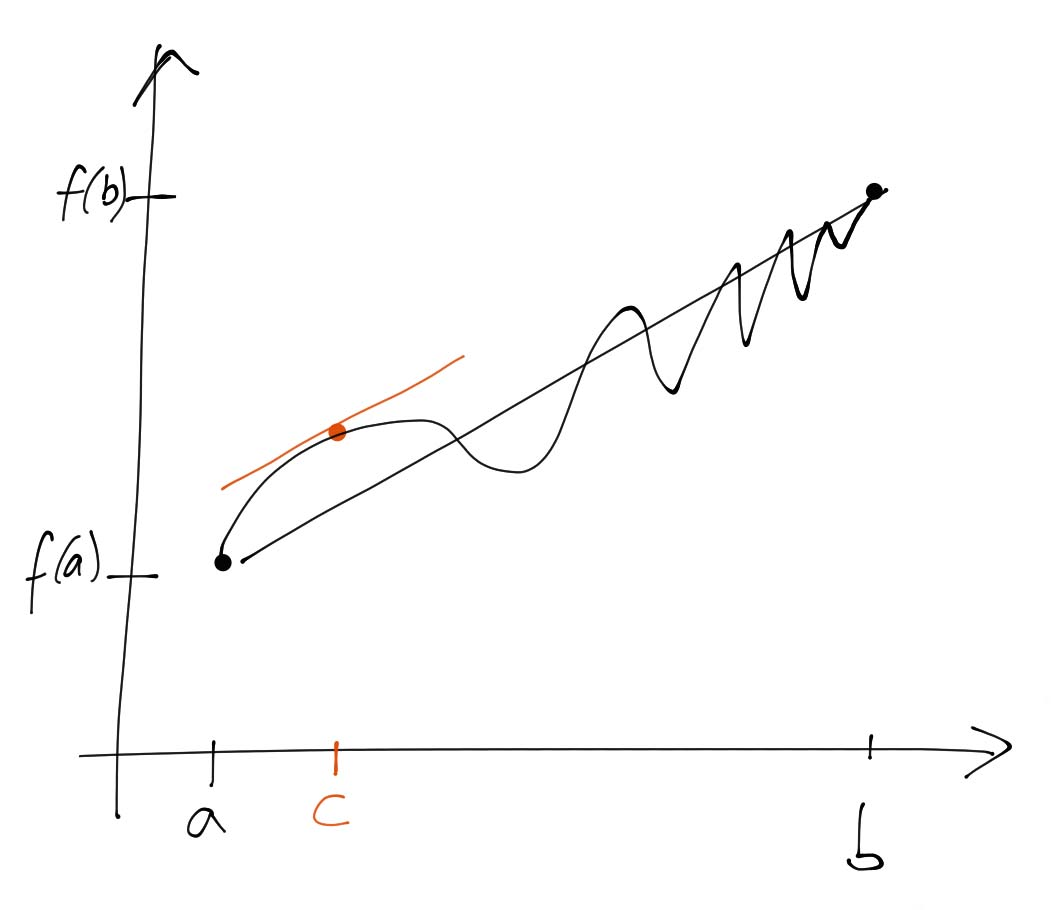
\includegraphics[width = 9cm]{mvt1.jpg}
\end{center}
Note: we can write this as $f(b) = f(a) + (b-a)f'(c)$, $c \in (a,b)$. Compare this to Taylor's Theorem - we're taking just the first $2$ terms of.

\emph{Idea of Proof:} Turn MVT into Rolle. 

\begin{center}
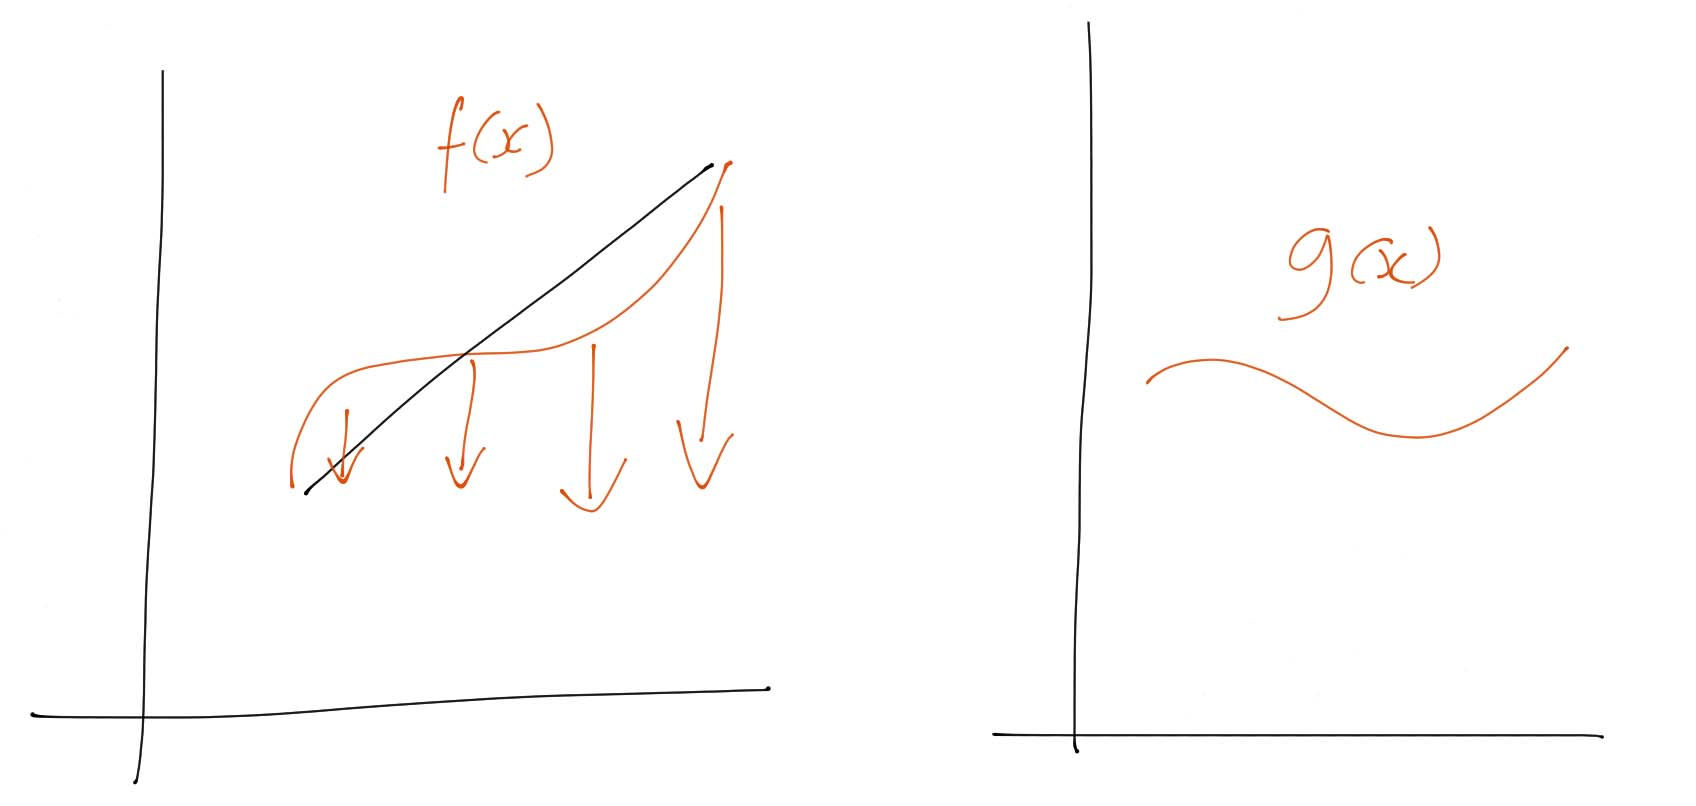
\includegraphics[width = 12cm]{mvt2.jpg}
\end{center}

\begin{proof}
Let $g(x) = f(x) - \dfrac{f(b) - f(a)}{b-a}(x-a)$, which is cts on $[a,b]$ and diff'ble on $(a,b)$. $g(a) = f(a) = g(b)$. By Rolle's Theorem applied to $g$
\[\exists c \in (a,b)\text{ such that }g'(c) = 0 \implies g'(c) = f'(c) - \dfrac{f(b) - f(a)}{b-a}.\qedhere\]	
\end{proof}\vspace*{5pt}

\begin{corollary}
If $f'(x) = 0~\forall x \in (a,b)$. Then $f$ is a constant: $f(x) = f(a)~\forall x \in [a,b]$
\end{corollary}
\begin{proof}
Suppose for a contradiction that $\exists d \in[a,b]$ s.t. $f(d) \neq f(a)$. Then by MVT applied to $\left. f\right|_{[a,d]}: [a,d] \to \RR$, $\exists c\in(a,d)$ s.t. $f'(c) = \dfrac{f(d) - f(a)}{d-a} \neq 0,~\cont$	
\end{proof}


\begin{theorem}[Chain Rule]\lecturemarker{28}{19 March} $g: \RR \to \RR$ diff'ble at $a \in \RR$, $f: \RR \to \RR$ diff'ble at $g(a) \in \RR$, then $f \circ g$ diff'ble at $a$ with $(f\circ g)'(a) =f'(g(a))g'(a)$
\end{theorem}

i.e. \[\left.\frac{d}{dx} f(g(x))\right|_{x=a} = \frac{df}{dx} (g(a)) \frac{dg}{dx}(a) = \left.\frac{df}{dy}\right|_{y=g(a)}\frac{dg}{dx}(a) ``=" \frac{df}{dg}\frac{dg}{dx}\]

\emph{Idea of proof:} 
\[\frac{f(g(x))-f(g(a))}{x-a} = \frac{f(g(x)) - f(g(a))}{g(x) -g(a)}\cdot\frac{g(x)-g(a)}{x-a} \to f'(g(a))\cdot g'(a)\]
problem with this is that $g(x) - g(a)$ might be zero

$\left(\dfrac{h(x) - h(a)}{x-a} \text{ is not defined at } x=a \text{, so define it to be } h'(a) \text{ at } x=a \right)$\\

\begin{proof}
Define $F(g) = \begin{cases}
 	\dfrac{f(y)-f(b)}{g-b} & y \neq b\\
 	f'(g) &  y = b 
 \end{cases}~(\ddagger)$
 where $b = g(a)$. \vspace*{5pt}\\$f$ is diff'ble at $b \implies \lim_{y \to b} F(y) \to f'(b) = F(b)$ as $y \to b$. So $F$ is cts at $b = g(a) ~(*)$. 
 
 $g$ is diff'ble at $a \implies$ cts at $a$. 
 
 By $(*) \implies F \circ g$ is cts at $a \implies F(g(x)) \to F(g(a)) = f'(b)$ as $x \to a ~(**)$. 
 
 So now we can follow the rough proof to write 
 \[\frac{f(g(x)) -f(g(a))}{x} = F(g(x))\frac{g(x) - g(a)}{x-a}\]
 

 
 Now take $\lim_{x\to a}$ to get $(f\circ g)'(a)$ exists and equals $f'(b)g'(a)$ by $(**)$ \end{proof}\vspace*{5pt}
 
 Ex: ``Sum Rule" $f, g$ are differentiable at $a\implies f+g$ are differentiable at $a$ with $(f+g)'(a) = f'(a) + g'(a)$. Pre-ex: Algebra of limit for $\lim_{x\to a}$ is on Question Sheet.\\
 
 \emph{Rough:} $f: \RR\to \RR$ is differentiable and bijective, $g = f^{-1}: \RR \to \RR$.
 
  Suppose $g$ is differentiable. Then by the chain rule $f\circ g(y) = y \implies f'(g(y_0))g'(y_0) = 1~\forall y_0 \implies g'(y) = \frac{1}{f'(g(y))}$. 
  
  Suggests that if $f' \neq 0$, then $g$ is differentiable with derivative $\frac{1}{f'\circ g}$\vspace*{5pt}

\begin{theorem}
	If $f:\RR \to \RR$ is differentiable at $a\in \RR$ with $f'(a) \neq 0$ and $f$ is bijective with inverse $g = f^{-1}$, then $g$ is differentiable at $b = f(a)$ with $g'(b) = \dfrac{1}{f'(g(b))} = \dfrac{1}{f'(a)}.$
\end{theorem}
\begin{proof}
\textit{Lemma:} $f'(a) \neq 0 \implies \exists \delta > 0$ such that $f(x) \neq f(a)$ for $x \in (a-\delta,a + \delta)\backslash\{0\}$.  (Proof is left as exercise - use $\lim_{x\to a}$ definition of $f'$ and MVT) \\

 So $\dfrac{g(y)-g(b)}{y-b} = \dfrac{x-a}{f(x) - f(a)} = 1/\dfrac{f(x)-f(a)}{x-a}$ where $x = g(y),~y \neq b$.
 
 As $y \to b$, $g(y) \to g(b) = a$ since $f$ differentiable at $a \implies f$ cts at $a \implies g$ cts at $b \implies x \to a \implies$ RHS $\to \dfrac{1}{f'(a)}$.	
\end{proof}\vspace*{15pt}



\textbf{Felina.} Suppose $f: \RR \to \RR$ satisfies
\begin{itemize}
\item $f(x) + f(y) = f(x+y)~\forall x,y\iR$
\item $f$ is continuous everywhere	
\end{itemize}

\emph{What if $f$?}

Observe $y = 0: f(x) + f(0) = f(x),~\forall x$, so $f(0) = 0$. 

For $y = 1: f(x) + f(1) = f(x+1)$

\[\begin{aligned}\text{Induction } f(x+2) &= f(x) + f(1) + f(1) \\
f(x+3) &= f(x) + 3f(1)\\
&\vdots \\ 
 f(x+n) &= f(x) + nf(1)\\
\implies f(n) &= nf(1) ~(*)\end{aligned}
\]

Similar mucking about should convince you that $f(x) = xf(1)$. We've proved that for $x\iN$ by $(*)$. $f(1)$ is an unknown constant $c$. [Notice $f(x) = cx$ indeed satisfies the given assumptions]

Notice \lecturemarker{29}{20 March} that $(*)$ holds for $n \iZ$ too
\[f(-n) + f(n) = f(n-n) = f(0) = 0\]
\[\implies f(-n) = -f(n) = -nf(1) = -nc,\quad n \iN\]
$(*)$ also holds for $\QQ$
\[\textstyle{\underbrace{\textstyle{f(\frac{n}{m}) + \dots + f(\frac{n}{m})}}_{m \text{ copies}} = f(\frac{n}{m} + \dots + \frac{n}{m}) =f(n) = cn}\]
\[\textstyle{\implies f(\frac{n}{m}) = c\frac{n}{m} \quad \forall \frac{n}{m} \iQ,~n,n\iZ}\]

\textbf{Claim:} $f(x) = cx$ [$c = f(1)$] $\forall x \iQ$

\emph{Idea:} now is if $x \iR$ then $x$ is close to $y \iQ$. $f$ is continuous $\implies f(x)$ is close to $f(y) = cy$, close to $cx$. So $f(x)$ is arbitrarily ($\forall \epsilon!$) close to $cx \implies f(x) = cx$

(or we could use some machinery to say $\forall x \iR$, $\exists (y_n) \to x$, $y_n \iQ$. Then $f$ is continuous $\implies f(y_n) = cy_n \to f(x)$ and $cy_n \to cx$. So uniqueness of limits $\implies f(x) = cx$.) 

\begin{proof}
Fix $x \iR$. Fix $\epsilon >0$. M1F: $\exists y \iQ$ s.t. $|y-x| < \epsilon \implies |cy - cx| < \epsilon/2$
\[\exists \delta >0\text{ s.t. }|x-y| < \delta \implies |f(x) - f(y)| < \epsilon/2\]

and by M1F again $\exists y\iQ$ s.t. $|y-x| < \mathrm{min}\{\delta,\epsilon/2\}$. 

So $|cy-cx|< \epsilon/2$ and $|f(x) - \equalto{f(y)}{cy}| < \epsilon/2 \implies |f(x) - cx| < 2\epsilon/2 = \epsilon$. 

This is true $\forall \epsilon >0 \implies |f(x) -cx| = 0$
\end{proof}



  \begin{center}
  \textsf{\textbf{- End of Analysis I -}}	
  \end{center}
  
  \stepcounter{lecture}
\setcounter{lecture}{1}

  